\documentclass{article}
\usepackage{graphicx}
\usepackage{subcaption}
\usepackage{geometry}
\usepackage{tikz}
\usepackage{amsmath}
\usepackage{cleveref}
\usepackage{float}
\usepackage[useregional]{datetime2}
\usepackage{url}
\def\checkmark{\tikz\fill[scale=0.4](0,.35) -- (.25,0) -- (1,.7) -- (.25,.15) -- cycle;}
\usepackage[font=small,skip=0pt]{caption}
\geometry{legalpaper, margin=1in}
\title{A Shallow Study on Rumble Strips' Effectiveness on Different Road Conditions}
\author{Zhijia Chen}
\date{\today}

\begin{document}

\begin{titlepage}
    \maketitle
\end{titlepage}

\section*{Summary}
Rumble strips has been widely adopted as an economic measure to alert inattentive drivers of potential dangers. A rumble strip is a raised or grooved pattern on travel lanes and has different texture with the road on with it is installed. When vehicle tires pass over the strip, they produce a sudden rumbling sound and cause the automobile to vibrate so as to alert inattentive or drowsy drivers[]. It is expected that drivers will pay more attention when passing the road and thus reduce the possibility of potential car accidents. A car accident is such a complex random event that contributed by many factors, it is hard to tell how effective rumble strips are in reducing crashes. So, in this study, we explore the effectiveness of rumble strips by comparing the changes in yearly car crashes number between roads with and without rumble installed in an observed time span (2004 to 2012). We find that there isn't strong evidence that rumble stripes have a general effects in reducing average number of crash on all roads. But when we focus on roads with certain condition, such as road curvature, road width, speed limit, etc., we found that on roads with curvature degree greater than 5, rumble strips can prevent \% of car crashes on average. We also find that rumble strips is also likely to reduce ?\% of car crashes on roads of width greater than 24 feet while they have positive effects in narrower roads, which is unexpected as by intuition we think a crash is more likely to happen if the road is narrower. By further investing the annual traffic volume, we realize that wider roads usually hold more traffic volume and thus higher car accident possibility. We also suspect that rumble strips would help on crash-prone roads, i.e., roads with car accident records in 2004, but we didn't find any strong evidence to support that. 

\section*{Dataset and Assumption}

This study works with the dataset "PennCrash.txt"[] that provides number of crashes occurred on about 2000 road segments (sites) in Pennsylvania in the year 2004, 2008 and 2012. Among these sites, rumble strips were installed in 331 of them between year 2008 and 2012. The dataset also gives some features of the roads including annual average daily traffic (AADT) volume, curvature, width, posted speed limit and so on. As we do not know if rumble stripes were installed in 2008 or not, we only use the data of the year 2004 and 2012, and we assume that by the beginning of 2012, all the rumble stripes in this dataset had been installed. Thus we have a clean data to study the crash number before and after rumble strips installation.

\section*{Methodology}

To study if rumble strips help in reducing the number of car crashes, a naive approach is to compare the car accident number before and after rumble strip installation. However, 8 years (2004 to 2012) is quite a long time span and many factors that affect car crash could have changed over time, such as better traffic control system, improved overall driving behavior, better car control system, higher/lower traffic volume, etc., and we cannot simply claim the changes in car crashes as being the effect of rumble stripes. So we take data of roads that do not have rumble strips treatment as a control group, and those that have rumble strips treatment as treat group. We will study the total crash number changes between year 2012 and year 2004 of the two groups, and test the differences between the two population. When investigating rumble strips' effects on roads of particular features, we will filter the data using the corresponding column before testing the differences. 

And to compare two population, we perform single-tailed two sample t-test to test their means are equal and get the p value. Generally, we have the following null hypothesis and alternative hypothesis:

\begin{align*}
    H_0: &Mean(tot12-tot04)|(treat, condition(f_1, f_2, ..., f_n)) >= \\
         &Mean(tot12-tot04)|(not treat, condition(f_1, f_2, ..., f_n))\\
    H_1: &Mean(tot12-tot04)|(treat, condition(f_1, f_2, ..., f_n)) < \\
         &Mean(tot12-tot04)|(not treat, condition(f_1, f_2, ..., f_n))\\
\end{align*}

Where $tot04$ and $tot12$ are the total number of crashes in year 2004 and 2012 respectively, and $Mean(tot12-tot04)|(treat, condition(f_1, f_2, ..., f_n))$ denotes the mean value of $tot12-tot04$ of roads that have rumble stripe treatment with conditions on road features $f_1, f_2, ..., f_n$. $H_0$ means rumble strips treatment has no effect or has reverse effect in reducing car crash number on roads with features safisfying $condition(f_1, f_2, ..., f_n)$. We set $\alpha$ value to 0.05 in this study.

\section*{Rumble Strips Effectiveness Tests}

We first study rumble strips' effects on all the roads in the dataset regardless of any road features. Figure ~\ref{fig:general-effect} shows the distribution of the two population. The mean value for the population with rumble strips treatment is -0.066 and 0.028 for that without treatment. While the mean value of the treatment group is slightly smaller than the control group, the p value is 0.057 so we accept the null hypothesis. But still, we can see that the distribution at 1 is marginally smaller than the value at -1 in the group with treatment, and the other way around in the other group. This is a good sign that we can find a more significant difference if we refine the two groups with certain condition on some road features.

\begin{figure}[h!]
    \centering
    \includegraphics[width=0.5\textwidth]{with-and-without-rumble-diff.png}
    \caption{distribution of tot12-tot04 on roads with and without rumble treatment}
    \label{fig:general-effect}
\end{figure}

Then we consider the roads of large curvature. We first check roads with curve degree greater than 3, the mean value of $tot12-tot04$ for the treat group is ? against ? for the control group, and the p value is ?, which rejects the null hyposthesis. When we further increase the curve degree threshold to 5, the difference is more significant, with the mean value difference increase to ? and p value decrease to ?. Figure ~\ref{fig:curve-grt3} and figure ~\ref{fig:curve-grt5} shows the distribution of $tot12-tot04$ of the two cases respectively. 

\begin{figure}[H]
    \centering
    \begin{subfigure}{.5\textwidth}
        \centering
        \includegraphics[width=1\textwidth]{with-and-without-rumble-curvature-grt3-diff.png}
        \caption{distribution of tot12-tot04 on roads of curve degree $>$ 3     with and without rumble treatment}
        \label{fig:curve-grt3}
    \end{subfigure}%
    \begin{subfigure}{.5\textwidth}
        \centering
        \includegraphics[width=1\textwidth]{with-and-without-rumble-curvature-grt5-diff.png}
        \caption{distribution of tot12-tot04 on roads of curve degree $>$ 5     with and without rumble treatment}
        \label{fig:curve-grt5}
    \end{subfigure}
    %\caption{A figure with two subfigures}
    %\label{fig:test}
\end{figure}

To test our model, we do a 1-year span forecast and compare it against the actual data. Figure ~\ref{fig:forecast1} presents the forecast data and the error. We notice that the change trend of the forecast generally matches the actual data, but the data change scale diminishes as the time goes which makes the future predication approaching to a constant. Figure ~\ref{fig:forecast10} shows a 10-year forecast and the predicated data indeed level off after 3 years. Overall, the results show that our model is capable of doing a good short term forecast but would need further improvements to increase the reliable forecast span.

\begin{figure}[H]
    \centering
    \includegraphics[width=0.5\textwidth]{forecast-1-year.jpg}
    \caption{1-year span forecast data and the forecast error}
    \label{fig:forecast1}
\end{figure}

\begin{figure}[H]
    \centering
    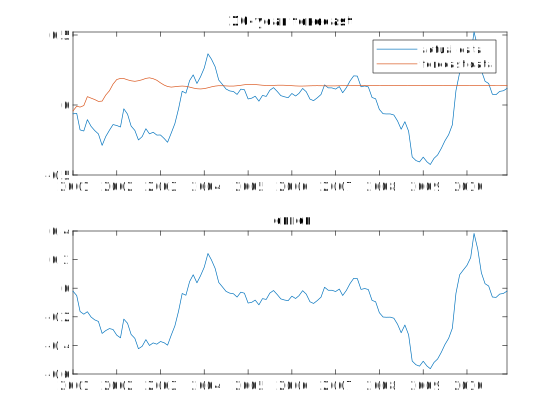
\includegraphics[width=0.5\textwidth]{forecast-10-year.jpg}
    \caption{1-year span forecast data and the forecast error}
    \label{fig:forecast10}
\end{figure}

\bibliography{project1} 
\bibliographystyle{ieeetr}
\end{document}

